%%%%%%%%%%%%%%%%%%%%%%%%%%%%%%%%%%%%%%%%%
% Short Sectioned Assignment
% LaTeX Template
% Version 1.0 (5/5/12)
%
% This template has been downloaded from:
% http://www.LaTeXTemplates.com
%
% Original author:
% Frits Wenneker (http://www.howtotex.com)
%
% License:
% CC BY-NC-SA 3.0 (http://creativecommons.org/licenses/by-nc-sa/3.0/)
%
%%%%%%%%%%%%%%%%%%%%%%%%%%%%%%%%%%%%%%%%%

%----------------------------------------------------------------------------------------
%	PACKAGES AND OTHER DOCUMENT CONFIGURATIONS
%----------------------------------------------------------------------------------------

\documentclass[paper=a4, fontsize=11pt]{scrartcl} % A4 paper and 11pt font size %
%\documentclass{standalone} %表格
\usepackage{multirow}      %表格
\usepackage{color}
\usepackage{comment}

\usepackage[T1]{fontenc} % Use 8-bit encoding that has 256 glyphs
%\usepackage{fourier} % Use the Adobe Utopia font for the document - comment this line to return to the LaTeX default
\usepackage[english]{babel} % English language/hyphenation
\usepackage{amsmath,amsfonts,amsthm, bm} % Math packages

\usepackage{graphicx} % Required for the inclusion of images

\usepackage{lipsum} % Used for inserting dummy 'Lorem ipsum' text into the template

\usepackage{sectsty} % Allows customizing section commands
\allsectionsfont{\centering \normalfont\scshape} % Make all sections centered, the default font and small caps
\usepackage{geometry}   %设置页边距的宏包
\geometry{left=2.5cm,right=2.5cm,top=2.5cm,bottom=2.5cm}  %设置 上、左、下、右 页边距
\usepackage{indentfirst} %设置首行缩进
\setlength{\parindent}{2em}

\usepackage{fancyhdr} % Custom headers and footers
\pagestyle{fancyplain} % Makes all pages in the document conform to the custom headers and footers %
\fancyhead{} % No page header - if you want one, create it in the same way as the footers below
\fancyfoot[L]{} % Empty left footer
\fancyfoot[C]{} % Empty center footer
\fancyfoot[R]{\thepage} % Page numbering for right footer
\renewcommand{\headrulewidth}{0pt} % Remove header underlines
\renewcommand{\footrulewidth}{0pt} % Remove footer underlines
\setlength{\headheight}{13.6pt} % Customize the height of the header
\setlength{\footheight}{13.6pt} % Customize the height of the header

\numberwithin{equation}{section} % Number equations within sections (i.e. 1.1, 1.2, 2.1, 2.2 instead of 1, 2, 3, 4)
\numberwithin{figure}{section} % Number figures within sections (i.e. 1.1, 1.2, 2.1, 2.2 instead of 1, 2, 3, 4)
\numberwithin{table}{section} % Number tables within sections (i.e. 1.1, 1.2, 2.1, 2.2 instead of 1, 2, 3, 4)

\def\bf{\normalfont\bfseries}
%\setlength\parindent{0pt} % Removes all indentation from paragraphs - comment this line for an assignment with lots of text

%----------------------------------------------------------------------------------------
%	TITLE SECTION
%----------------------------------------------------------------------------------------

\newcommand{\horrule}[1]{\rule{\linewidth}{#1}} % Create horizontal rule command with 1 argument of height


\title{	
\normalfont \normalsize
\textsc{University of Universe, Department of Earth} \\ [24pt] % Your university, school and/or department name(s)
\horrule{0.5pt} \\[0.4cm] % Thin top horizontal rule
\huge{\textbf{ETH AAA}} \\ % The assignment title
\textbf{ Report on Colabration with Cybertron }\\[0.5cm]
%\horrule{1pt} \\[0.75cm] % Thick bottom horizontal rule
}

\author{ \LARGE{\texttt{Firstname \textsc{Lastname}, ID: 12345678}}\\
\normalfont \normalsize {x001@abc.com} \\
} % Your name

\date{{December 8, 2016}} % Today's date or a custom date
%\Large{} \\
%\Large{\textit{Prepared for: Dr. Awesome}}\\


\makeatletter
\renewcommand{\section}{\@startsection{section}{1}{0mm}
  {-\baselineskip}{1\baselineskip}{\bf\leftline}}
\makeatother

\makeatletter %左对齐
\renewcommand{\subsection}{\@startsection{subsection}{1}{2mm}
  {-\baselineskip}{0.5\baselineskip}{\bf\leftline}}
\makeatother

\makeatletter %左对齐
\renewcommand{\subsubsection}{\@startsection{subsubsection}{1}{4mm}
  {-\baselineskip}{0.5\baselineskip}{\bf\leftline}}
\makeatother

\begin{document}

\begin{titlepage}
\maketitle
\end{titlepage}
%\maketitle % Print the title
%----------------------------------------------------------------------------------------
%	TASK 1
%----------------------------------------------------------------------------------------

\section{Introduction}
\lipsum[1]

\section{Relationship}\label{Sec:LS}
\lipsum[2]


\subsection{Comparison between A and B}

\begin{enumerate}
\renewcommand{\labelenumi}{(\theenumi)}
\item Similarities.
\lipsum[1]

\item Differences.
\lipsum[1]
\end{enumerate}



\subsection{HO in Dealing with Robots}
Humor origin \cite{mcghee1979humor}.


\subsubsection{Blabla}
\lipsum[1]

\begin{table}[!htbp]
  \centering
  \caption{What is this}\label{tab:Task2}
\begin{tabular}{|l|c|c|c|c|c|c|}
  \hline
  % after \\: \hline or \cline{col1-col2} \cline{col3-col4} ...
   & $\epsilon_{P_E}$(m) & $\epsilon_{P_N}$(m) & $\epsilon_{P_U}$(m) & $\epsilon_{V_E}$(m/s) & $\epsilon_{V_N}$(m/s) & $\epsilon_{V_U}$(m/s) \\\hline
  P $\& \dot{P}$ ($q_v$ = 50)
  & 0.0146  &  0.0268  &  0.0359  &  0.0255   & 0.0243 &   0.0007 \\ %q = 50 PP.
  P $\& \dot{P}$ ($q_v$ = 20)
   &$\bm{0.0156}$   & $\bm{0.0327}$   &  $\bm{0.0359}$    & $\bm{0.0254}$   &  $\bm{0.0240}$    & $\bm{0.0007}$  \\%q = 20 PP.
  P $\& \dot{P}$ ($q_v$ = 10)
   & 0.0187  &  0.0430  &  0.0359  &  0.0251 &   0.0235  &  0.0007 \\%q = 10 PP.
  P $\& \dot{P}$ ($q_v$ = 0.1)
   & 0.1105 &   0.1823  &  0.0357  &  0.0405   & 0.1846  &  0.0007 \\\hline%q = 0.1 PP.
  P ($q_v = 50 $)
  & 0.0422  &  0.0826  &  0.0345   & 0.9267   & 1.0108  &  0.0008 \\ %q = 50 P
  P ($q_v = 20 $)
   &0.0465  &  0.1055  &  0.0345   & 0.9729  &  1.1492   & 0.0008 \\ %q = 20 P
  P ($q_v = 10 $)
   & 0.0588 &   0.1562  &  0.0345  &  1.0429  &  1.3351  &  0.0008 \\ %q = 10 P
  P ($q_v = 0.1 $)
   & 1.2669  &  2.1024 &   0.0343  &  3.2233  &  3.8420  &  0.0023  \\ %q = 0.1 P
  \hline
\end{tabular}
\end{table}


\begin{table}[!htbp]
  \centering
  \caption{Seems good}\label{tab:Task3}
\begin{tabular}{|l|c|c|c|c|c|c|}
  \hline
  % after \\: \hline or \cline{col1-col2} \cline{col3-col4} ...
   & $\epsilon_{P_E}$(m) & $\epsilon_{P_N}$(m) & $\epsilon_{P_U}$(m) & $\epsilon_{V_E}$(m/s) & $\epsilon_{V_N}$(m/s) & $\epsilon_{V_U}$(m/s) \\\hline
  item1
   &$\bm{0.0197}$  &  $\bm{0.0544}$  & $\bm{ 0.0794} $  & $\bm{0.0253}$ &  $\bm{ 0.0258 } $& $\bm{ 0.0367}$ \\%q = 20 PP.
  item2
   & $\bm{0.0145}$  &  $\bm{0.0346}$    & $\bm{0.0793}$    & $\bm{0.0252}$  &   $\bm{0.0256}$  &   $\bm{0.0367}$ \\%q = 20 PP.
  %\parbox{10em}{ \\ }
  {item3}
  &\textcolor{blue}{$\bm{0.0156}$}  & \textcolor{blue}{$\bm{0.0327}$}   &  \textcolor{blue}{$\bm{0.0359}$}    & \textcolor{blue}{$\bm{0.0254}$}   &  \textcolor{blue}{$\bm{0.0240}$}    & \textcolor{blue}{$\bm{0.0007}$} \\%q = 20 PP.
  item4
   & $\bm{1.0011}$  &  $\bm{0.9520}$  &  $\bm{0.0358}$   & $\bm{0.0705}$  &  $\bm{0.3293}$  &  $\bm{0.0053}$ \\%q = 10 PP.
  \hline
\end{tabular}
\end{table}


\subsubsection{Matrix}
\lipsum[1]

\begin{equation}\label{Eq:Ft_10D}
  F =
  \begin{bmatrix}
        0_{3\times3} & I_{3\times3} & 0_{3\times4} \\
        0_{3\times3} & 0_{3\times3} & \left(
                                          \begin{array}{cccc}
                                            0 & 0 & 1 & 0 \\
                                            0 & 0 & 0 & 1 \\
                                            0 & 0 & 0 & 0 \\
                                          \end{array}
                                      \right)
         \\
        0_{2\times3} & 0_{2\times3} & \left(
                                        \begin{array}{cccc}
                                            0 & 1 & 0 & 0 \\
                                            0 & 0 & 0 & 0 \\
                                        \end{array}\right)
        \\
        0_{2\times3} & \left(\begin{array}{ccc}
                         -(\beta^2 + \omega^2) & 0 & 0 \\
                         0 & -(\beta^2 + \omega^2) & 0 \\
                       \end{array} \right)
                       & \left(\begin{array}{cccc}
                                       0 & 0 & -2\beta & 0 \\
                                       0 & 0 & 0 & -2\beta \\
                                     \end{array}\right)\\
  \end{bmatrix}
\end{equation}

\lipsum[1]
\begin{equation}\label{Eq:Gt_10D}
  G =
  \begin{bmatrix}
        0_{3\times5} \\
        \left(
          \begin{array}{ccccc}
            1 & 0 & 0 & 0 & 0 \\
            0 & 1 & 0 & 0 & 0 \\
            0 & 0 & 0 & 0 & 0 \\
            0 & 0 & 0 & 1 & 0 \\
            0 & 0 & 0 & 0 & 1 \\
          \end{array}
        \right)
         \\
        \left(
          \begin{array}{ccccc}
            \sqrt{\omega} & 0 & 0 & 0 & 0 \\
            0 & \sqrt{\beta} & 0 & 0 & 0 \\
          \end{array}
        \right)
  \end{bmatrix}
\end{equation}

\subsubsection{figure}
\lipsum[1]

\begin{comment}
\begin{figure}[!htbp]
  \begin{minipage}[t]{0.5\linewidth}
    \centering
    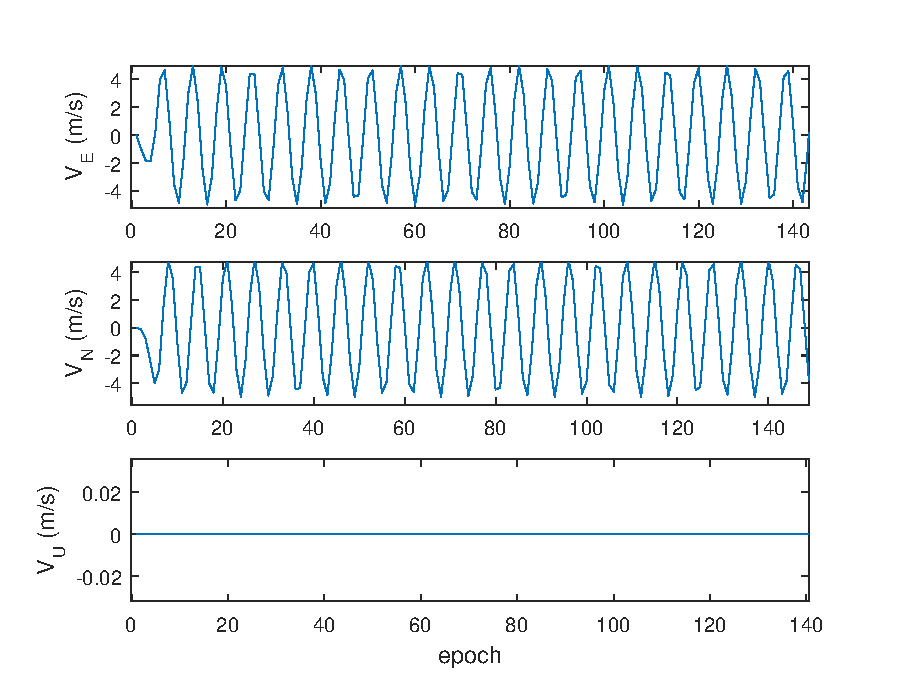
\includegraphics[width=3.0in]{Figures/SimuVel.eps}
    \caption{True Velocity}
    \label{fig:Simu_Vel}
  \end{minipage}%
  \begin{minipage}[t]{0.5\linewidth}
    \centering
    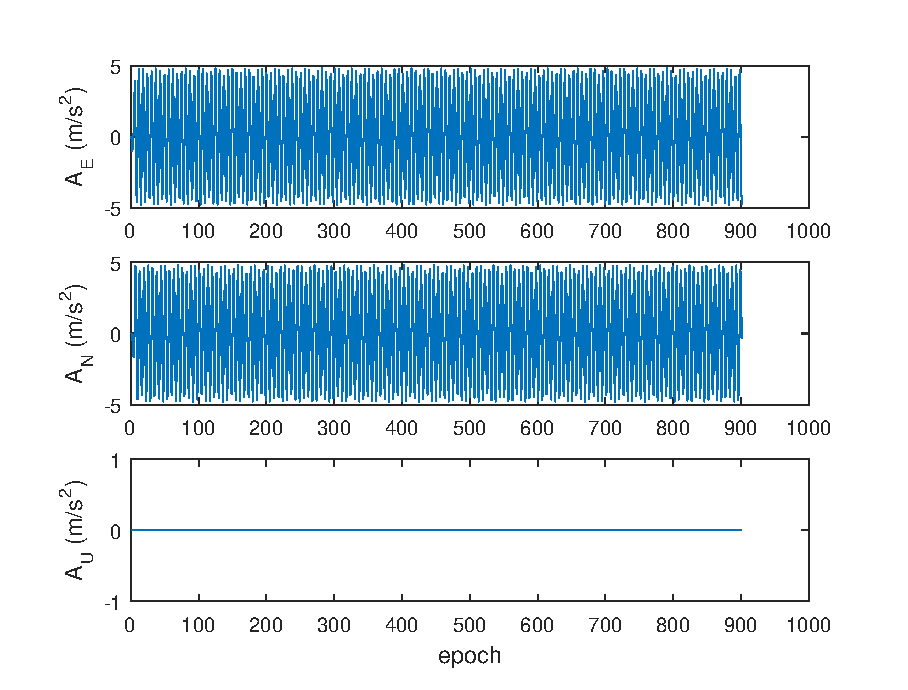
\includegraphics[width=3.0in]{Figures/SimuAcc.eps}
    \caption{True Acceleration}
    \label{fig:Simu_Acc}
  \end{minipage}
\end{figure}
\end{comment}

\renewcommand\refname{Reference}
\bibliographystyle{unsrt}
\bibliography{Report}

\end{document}

